\documentclass{szzclass}
\usepackage[czech]{babel}

\subject{DBS}
\code{BI-SPOL-11}
\topic{3 úrovně pohledu na data (konceptuální, implementační, fyzická). Struktury pro ukládání dat v relačních databázích s ohledem na rychlý přístup k nim (speciální způsoby uložení, indexy apod.)}

\begin{document}

\tableofcontents
\newpage

\section{3 úrovně pohledu na data}
\begin{figure}[h!]
  \centering
  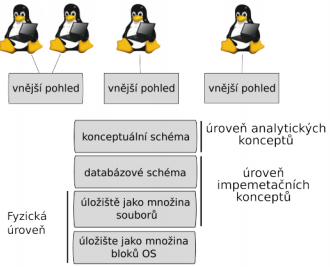
\includegraphics[width = \textwidth]{topics/bi-spol-11/images/views.png}
\end{figure}
\begin{description}
  \item[Konceptuální] Modelování reality (Obvykle se zachycuje se UML diagramem nebo ER modelem). Snaží se nebýt ovlivněna prostředky řešení.
  \item[Implementační] Konkrétní databázový model, konstrukční dotazovací a manipulační prostředky (relační, objektová, síťová, hierarchická, XML, \dots)
  \item[Fyzická] Sekvenční soubory, indexy, clustery apod.
\end{description}

\section{Konceptuální modelování databází}
\begin{itemize}
  \item společné chápání objektu aplikace uživateli a projektanty
  \item integrace několika uživatelských pohledů
  \item výsledek je vstupem do realizace DB
  \item slouží jako dokumentace
\end{itemize}

\section{Implementační}
\begin{itemize}
  \item nejnižší míra abstrakce
  \item v této fázi probíhá realizace datové struktury, popsané v konceptuálním modelu
  \item model je zde transformován do modelu odpovídající konkrétní technologii
  \item musí zohledňovat všechny dostupné prostředky a možnosti
  \item popisuje, čím je datový obsah systému, popsaný konceptuálním a strukturálním modelem, realizován
\end{itemize}

\section{Fyzický pohled}
\subsection{Struktury pro ukládání dat v relačních DB s ohledem na rychlý přístup k nim (speciální způsoby uložení, indexy apod.)}
\subsubsection{Heap}
\begin{itemize}
  \item nové záznamy přidány do libovolného prázdného místa
  \item žádné uspořádání
  \item hledání je O(n)
\end{itemize}
\subsubsection{Heap s indexy}
\begin{itemize}
  \item záznamy jsou uspořádány
  \item víme, když už můžeme ukončit hledání
\end{itemize}
\subsubsection{Cluster index}
\begin{itemize}
  \item index pages
  \item struktura už obsahuje samotné záznamy
  \item můžeme mít jenom jeden clustered index nad stejnými daty
\end{itemize}
\subsubsection{Noncluster index}
\begin{itemize}
  \item ukazatele do samotných záznamů
  \item libovolná organizace indexu (ROW ID)
\end{itemize}
\subsubsection{Bitmapové indexy}
\begin{itemize}
  \item binární matice
  \item předem vypočítané odpovědi na jednoduché otázky (true/false), a to pro každý záznam
  \item DLM operace velmi drahé
  \item spíš pro DSS (ne OLTP)
  \item vhodné pro záznamy s velmi neunikátními položkami
\end{itemize}
DSS = decission support system - velká rozhodnutí, založena na historických datech \newline
OLTP = online transaction processing - aktuální data, každodenní transakce
\subsubsection{Shluk}
Tabulky dané do jednoho shluku.
\begin{figure}[h!]
  \centering
  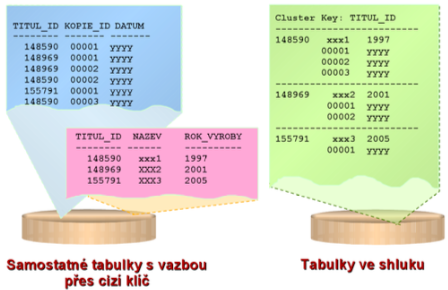
\includegraphics[width = \textwidth]{topics/bi-spol-11/images/cluster.png}
\end{figure}

\subsubsection{Index typu B*-Tree}
\begin{figure}[h!]
  \centering
  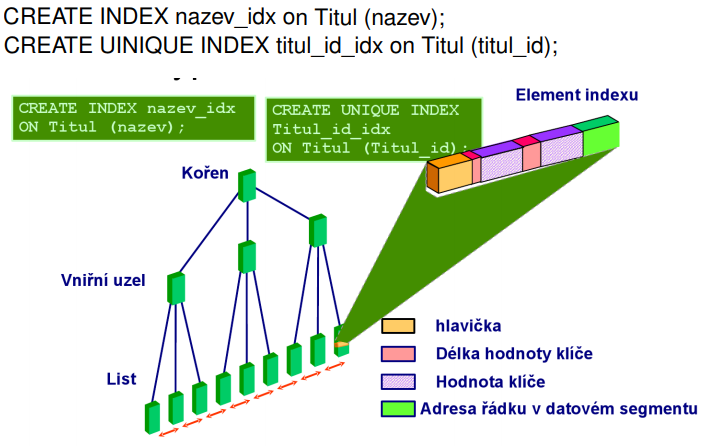
\includegraphics[width = \textwidth]{topics/bi-spol-11/images/bTree.png}
\end{figure}
\begin{itemize}
  \item kořen má nejméně 2 potomky, pokud není listem
  \item každý uzel kromě kožene a listu má nejméně [m/2] a nejvýše m potomků
  \item každý uzel má nejméně [m/2] - 1 a nejvíce m - 1 datových záznamů
  \item všechny cesty ve stromě jsou stejně dlouhé
  \item data v nelistovém uzlu jsou organizována
  \item listy obsahují úplnou množinu klíču a mohou se lišit strukturou
\end{itemize}
\section{Důležité poznatky}
\begin{itemize}
  \item (relační) databáze bez indexu nefungují rozumně - indexy jsou nutné (pro větší data)
  \item DB stroj často některé indexy vytváří automaticky kvůli kontrole IO (integritní omezení)
  \item v OLTP se nejčastěji používají indexy na bázi B-stromů (tam kde jsou data unikátní)
  \item kde jsou data velmi neunikátní a potřebují se indexovat, tam se používají bitmapové indexy
  \item indexy je třeba udržovat (zjednodušeně - ušetřím na dotazech, platím více při DML)
  \item klič indexu (indexované atributy) může být složený
  \item index může být unikátní/neunikátní
\end{itemize}
\end{document}
